\ifdefined\maindoc
\else
\documentclass[12pt]{report}
\usepackage[a4paper,left=40mm,right=25mm,top=25mm,bottom=25mm]{geometry}
\usepackage[utf8]{inputenc}
\usepackage[T1]{fontenc}
\usepackage[british]{babel}
\usepackage{amsmath,amssymb}
\usepackage{booktabs}
\usepackage{setspace}
\usepackage{graphicx}
\usepackage{enumitem}
\usepackage{placeins}
\usepackage{hyperref}
\usepackage[backend=biber,style=ieee,citestyle=numeric-comp,sorting=none]{biblatex}
\addbibresource{../../references.bib}
\onehalfspacing
\graphicspath{{figures/}}
% Standalone-only fallbacks. Numbering: 1 Introduction, 2 Background, 3 Network Model,
% 4 Network Decomposition, 5 Probability, 6 Capacity Flow, 7 Critical Path, 8 Julia package,
% 9 this chapter, 10 Integrated Case Study, 11 Conclusions.
\makeatletter
\newlabel{ch:main-intro}{{1}{1}{}{Doc-Start}{}}
\newlabel{ch:lit-review}{{2}{1}{}{Doc-Start}{}}
\newlabel{ch:system-model}{{3}{1}{}{Doc-Start}{}}
\newlabel{ch:diamond-module}{{4}{1}{}{Doc-Start}{}}
\newlabel{ch:probability-toolkit}{{5}{1}{}{Doc-Start}{}}
\newlabel{ch:capacity-toolkit}{{6}{1}{}{Doc-Start}{}}
\newlabel{ch:critical-path}{{7}{1}{}{Doc-Start}{}}
\newlabel{ch:julia-package}{{8}{1}{}{Doc-Start}{}}
\newlabel{ch:integrated-case-study}{{10}{1}{}{Doc-Start}{}}
\newlabel{ch:conclusions}{{11}{1}{}{Doc-Start}{}}
\makeatother
\begin{document}
\title{The No-Code Web Interface}
\fi

\section{Introduction}
\label{sec:fe-intro}

Chapter~\ref{ch:lit-review} closed on a gap that has nothing to do with algorithms. The
analyses of Chapters~\ref{ch:probability-toolkit} to~\ref{ch:critical-path} exist as a Julia
package, and a package is used by writing code. The engineer who holds the system model
does not write code. The tools that do reach such a person are either cloud
services, which are not acceptable for a proprietary system model, or licensed desktop
suites that carry none of these analyses.
That gap is closed by the interface described here. It is a browser application that
runs on the engineer's own machine, takes the same files the package reads, runs the three
toolkits against them through the local server of Chapter~\ref{ch:julia-package}, and
returns every result in the form the package computed it.

Each decision in the interface is described with the reason behind it.
Section~\ref{sec:fe-user} states who the interface is for and what follows from that.
Section~\ref{sec:fe-workflow} walks through the workflow in the order a user meets it, with
the screens of the power distribution network of Chapter~\ref{ch:probability-toolkit}
shown as illustrations of the controls. Section~\ref{sec:fe-rules} lists the rules the
interface enforces on how results are shown, and one rule it does not yet enforce.
Section~\ref{sec:fe-architecture} gives the architecture and Section~\ref{sec:fe-contract}
the contract between the interface and the package. Section~\ref{sec:fe-evaluation} states
what evidence the chapter can offer for usability and what it cannot, and
Section~\ref{sec:fe-limitations} the limits of the interface. The full application of the
interface to a real network, with results, is the subject of
Chapter~\ref{ch:integrated-case-study}; nothing in this chapter reports a number from a
screen.

\section{Who the Interface Is For}
\label{sec:fe-user}

An engineer with a system model and a question is the user. The model may be an edge list exported from an asset register or drawn up by hand. The
question is one of the three of Chapter~\ref{ch:main-intro}: with what probability does
supply reach this point, how much can the system deliver, or when does this sequence
complete. The user is assumed to know
the system and its data, to be comfortable with a spreadsheet and a browser, and not to
program.

Four requirements follow. The user must not have to write code, so every analysis is
reached by uploading files and pressing a button. The user must not have to learn a second
data format, so the files the interface accepts are the files the package reads, byte for
byte. The user's system model must not leave the user's machine, since the models in
question describe critical infrastructure and in some sectors cannot be sent to a third
party at all, so the interface runs against a local server and nothing is transmitted
elsewhere. And the user must be able to trust what is on the screen, so the interface shows
what the package computed and adds no interpretation of its own. The last requirement is
the one that shapes the interface most, and Section~\ref{sec:fe-rules} returns to it.

\section{The Workflow}
\label{sec:fe-workflow}

A session begins with an upload (Figure~\ref{fig:fe-upload}). The user selects a folder
that holds the network's structure file at its root and one sub-folder per scenario, each
scenario carrying any subset of the four input files of Chapter~\ref{ch:system-model}. The
upload page reads the folder before anything is sent and lists what it found: the network
name, the structure file, the scenarios, and for each scenario which toolkits its files
support and in which value form. A scenario folder may be named for its value form
(\texttt{float}, \texttt{interval}, \texttt{pbox}) or for an operating case
(\texttt{Baseline}, \texttt{Degraded}); in the second case the value form is read from
each file's own \texttt{data\_type} field. The expected layout is printed beside the
chooser, so that a user with a folder in the wrong shape sees the difference before
uploading.

\begin{figure}[htbp]
  \centering
  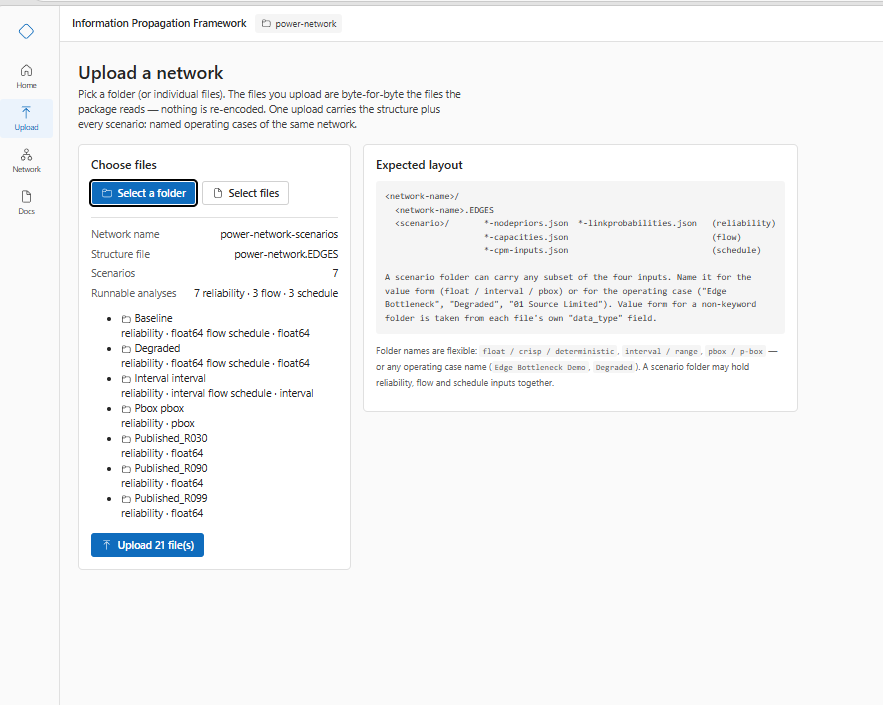
\includegraphics[width=0.85\linewidth]{fig01_upload/fig01_upload.png}
  \caption{The upload page. Left, the folder chosen, with the scenarios it holds and the
  analyses each supports listed before upload. Right, the expected folder layout.}
  \label{fig:fe-upload}
\end{figure}

On upload the server creates a session, a folder holding the files as uploaded and a
metadata record, and returns the network's structure. Figure~\ref{fig:fe-pipeline} gives the
shape of the whole workflow before the screenshots that follow walk through it step by
step. The network page (Figure~\ref{fig:fe-network}) shows the graph object of
Chapter~\ref{ch:system-model} as the package built it: node and edge counts, sources and
sinks, forks and joins, the layered order, and the network drawn by layer. This page is
where a user first sees whether the structure file was read as intended, since a
mis-oriented edge or a missing node shows here as a wrong source or an unexpected layer.

\begin{figure}[htbp]
  \centering
  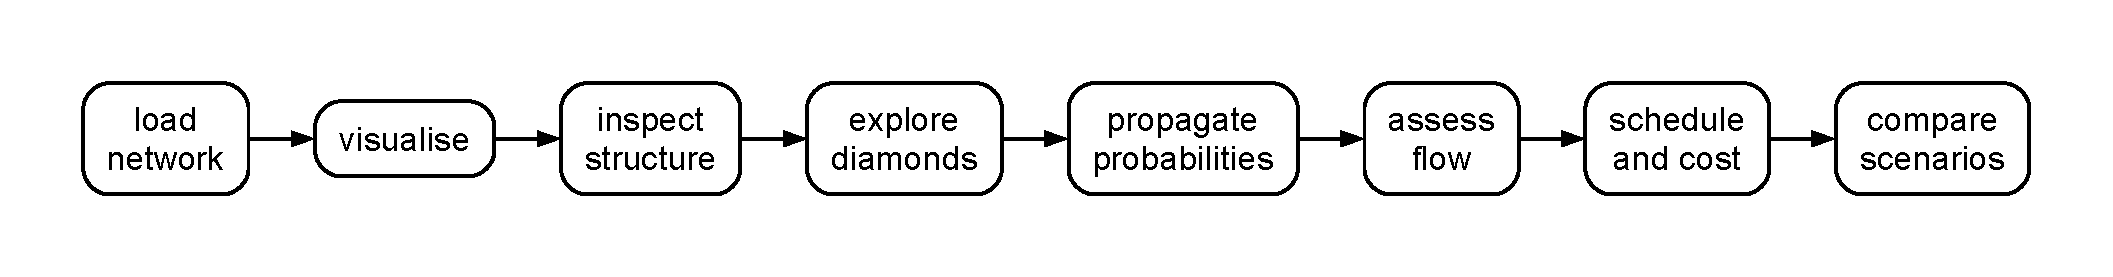
\includegraphics[width=\linewidth]{fig00_pipeline/fig00_pipeline.pdf}
  \caption{The workflow a session follows: load the network, then read its structure,
  explore its reconvergence, and apply the three toolkits, before comparing scenarios.}
  \label{fig:fe-pipeline}
\end{figure}

\begin{figure}[htbp]
  \centering
  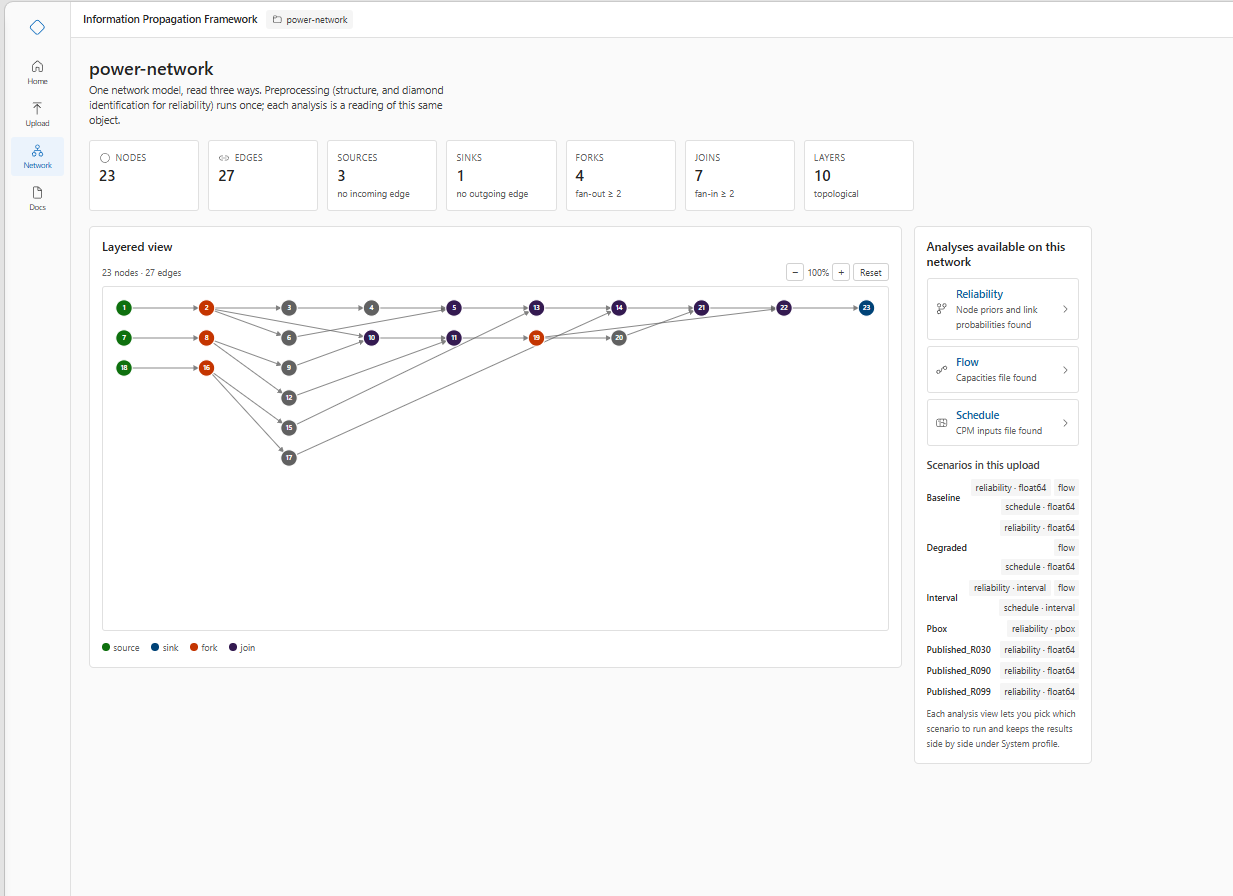
\includegraphics[width=0.9\linewidth]{fig02_network/fig02_network.png}
  \caption{The network page after upload: structural summary of the graph object and the
  network drawn by layer.}
  \label{fig:fe-network}
\end{figure}

Each toolkit has a page of its own, reached from the navigation rail, and the three pages
share one layout. A row of scenario chips at the top selects the scenario, each chip showing
the scenario's value form, and a value-form filter above the chips narrows the row to
deterministic, interval or probability-box scenarios. Below the chips are the toolkit's
tabs. For the probability toolkit (Figure~\ref{fig:fe-reliability}) these are Belief, the
per-node table with summary tiles; Diamonds, the reconvergence structure the decomposition
identified; Visualisation, the network drawn with the conditioning set highlighted; and
Compare. The Belief table can be filtered by node role and restricted to diamond joins, and
every summary tile names what it summarises. Similarly, the flow and schedule pages have
their own tabs: configuration, summary, bottlenecks and visualisation for flow
(Figure~\ref{fig:fe-flow}); time, cost, visualisation and compare for schedule
(Figure~\ref{fig:fe-schedule}).

\begin{figure}[htbp]
  \centering
  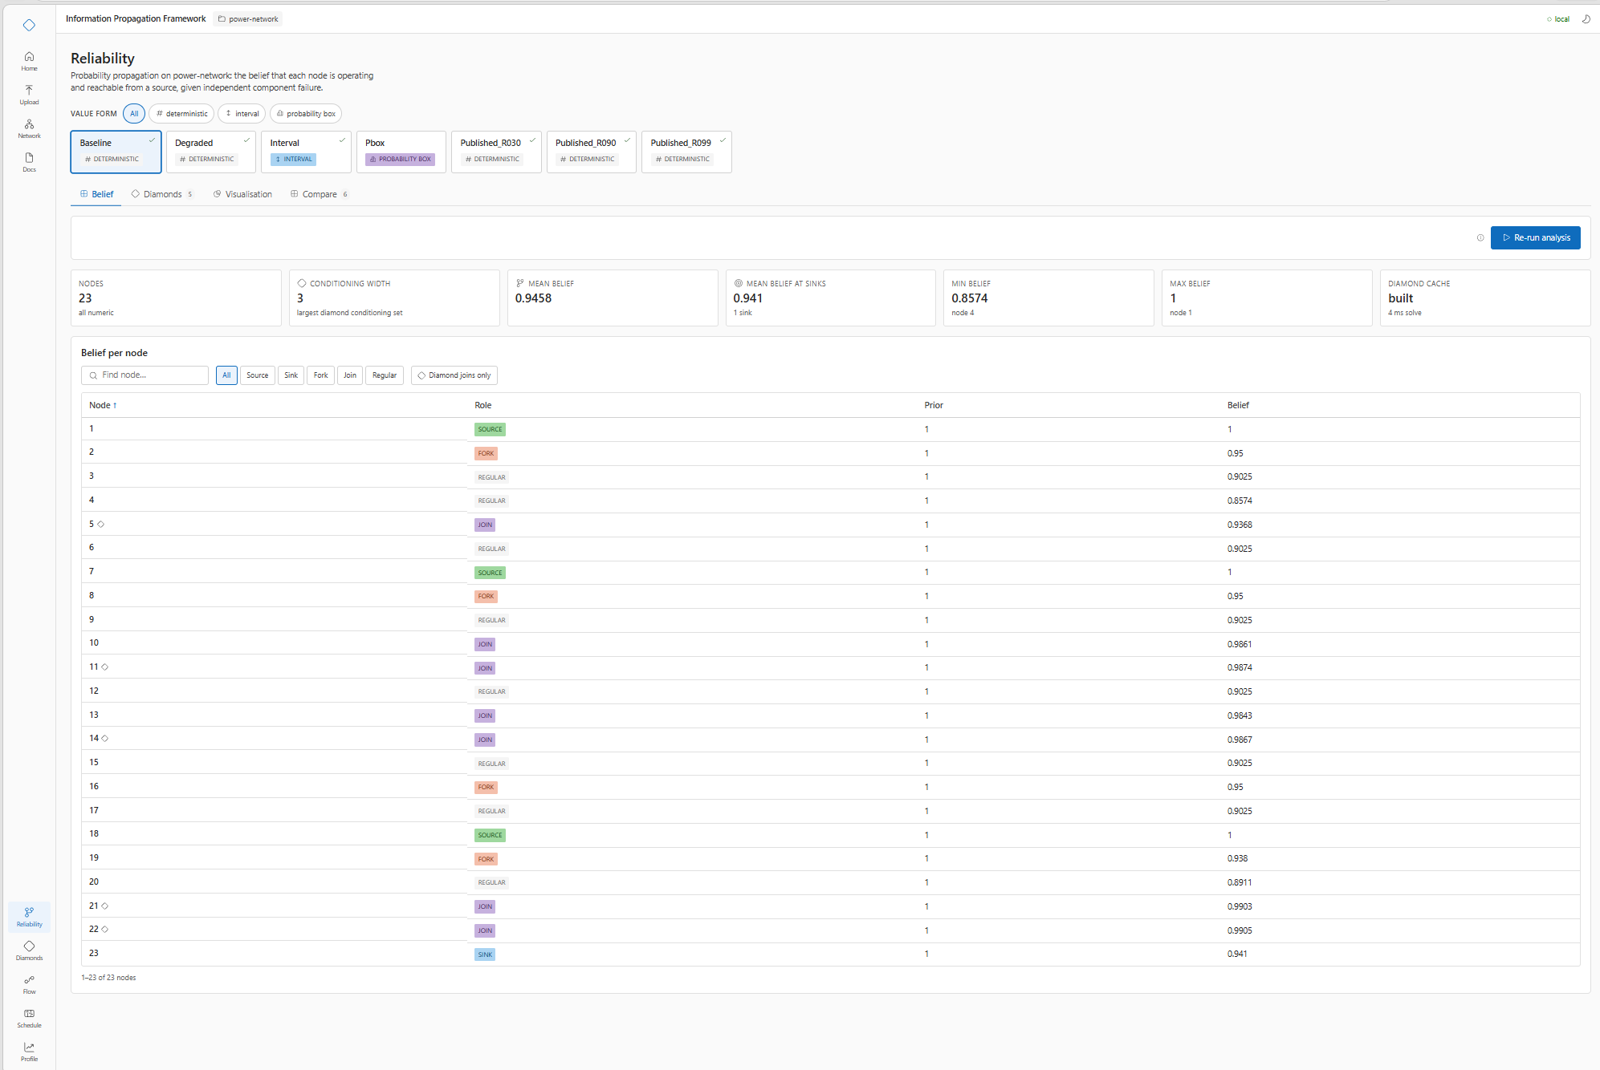
\includegraphics[width=\linewidth]{fig03_reliability_belief/fig03_reliability_belief.png}
  \caption{The reliability page, Belief tab. Top, the value-form filter and the scenario
  chips, each chip labelled with its value form. Below the tabs, summary tiles and the
  per-node belief table with its role filters.}
  \label{fig:fe-reliability}
\end{figure}

A diamond in the Diamonds tab opens a detail view (Figure~\ref{fig:fe-diamond}) that draws
the diamond as a graph of its own, lists its conditioning set, local sources and size, and
offers two actions. The first runs the reliability analysis on the diamond alone, as a
standalone network, with the local sources' priors overridable, which lets a user study a
reconvergence that dominates the network's uncertainty without the rest of the network in
view. The second promotes the diamond: it is uploaded as a new, independent network and
becomes a session of its own. Both actions are possible because Chapter~\ref{ch:diamond-module}
returns every diamond as a graph object of the same form as the network.

\begin{figure}[htbp]
  \centering
  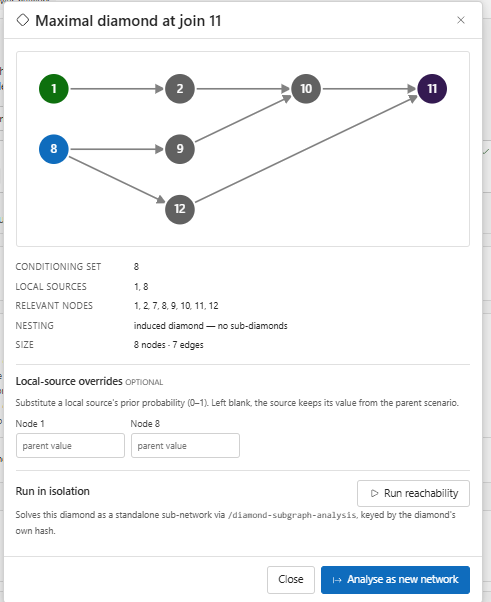
\includegraphics[width=0.55\linewidth]{fig04_diamond_detail/fig04_diamond_detail.png}
  \caption{A diamond's detail view: the subgraph, its conditioning set and local sources,
  the override fields for the local sources, and the two actions, run in isolation and
  analyse as a new network.}
  \label{fig:fe-diamond}
\end{figure}

\begin{figure}[htbp]
  \centering
  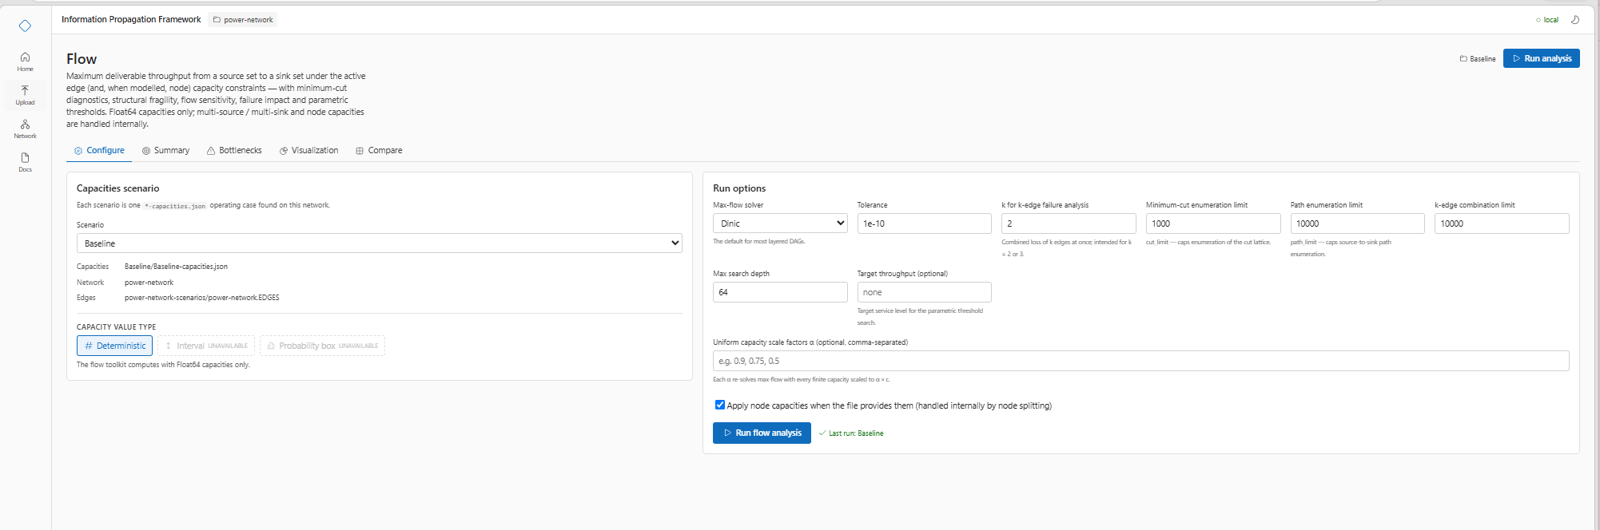
\includegraphics[width=\linewidth]{fig06_flow_config/fig06_flow_config.png}
  \caption{The flow page, configuration tab: scenario, solver, tolerance, the failure
  combination size, enumeration limits, and the optional target throughput and degradation
  multipliers.}
  \label{fig:fe-flow}
\end{figure}

\begin{figure}[htbp]
  \centering
  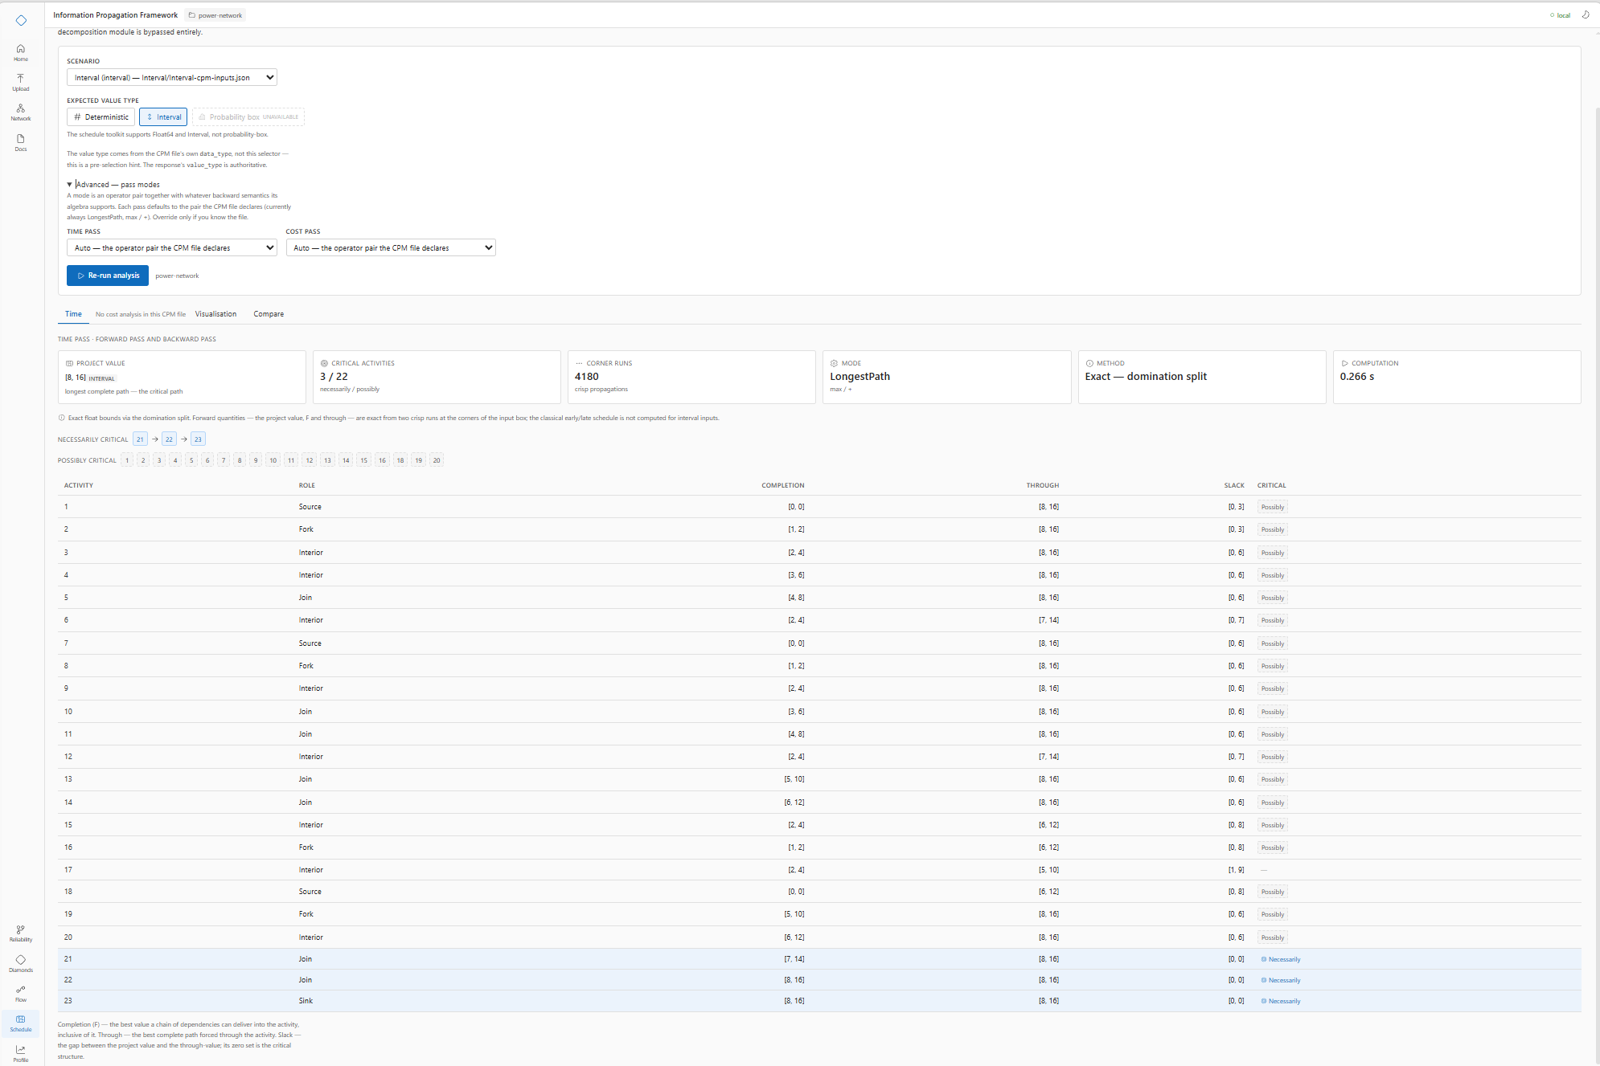
\includegraphics[width=\linewidth]{fig05_schedule_interval/fig05_schedule_interval.png}
  \caption{The schedule page under an interval scenario. The value-form selector shows the
  form the file declares and marks the probability-box form unavailable for this toolkit;
  the advanced control exposes the pass modes; the result tiles carry the method tag.}
  \label{fig:fe-schedule}
\end{figure}

The Compare tab (Figure~\ref{fig:fe-compare}) selects any subset of the network's scenarios
for the toolkit, runs those not yet run, one at a time, and places the results side by side
in one table with an optional baseline for differences. The system-profile page
(Figure~\ref{fig:fe-profile}) is the one view that crosses toolkits: every result set that
any analysis has produced on the network is listed, and any one of them can be drawn on the
network with a second overlaid, so that a schedule's critical path and a flow's binding cut
can be seen on the same nodes. The page computes nothing; it draws what the analyses
already found.

\begin{figure}[htbp]
  \centering
  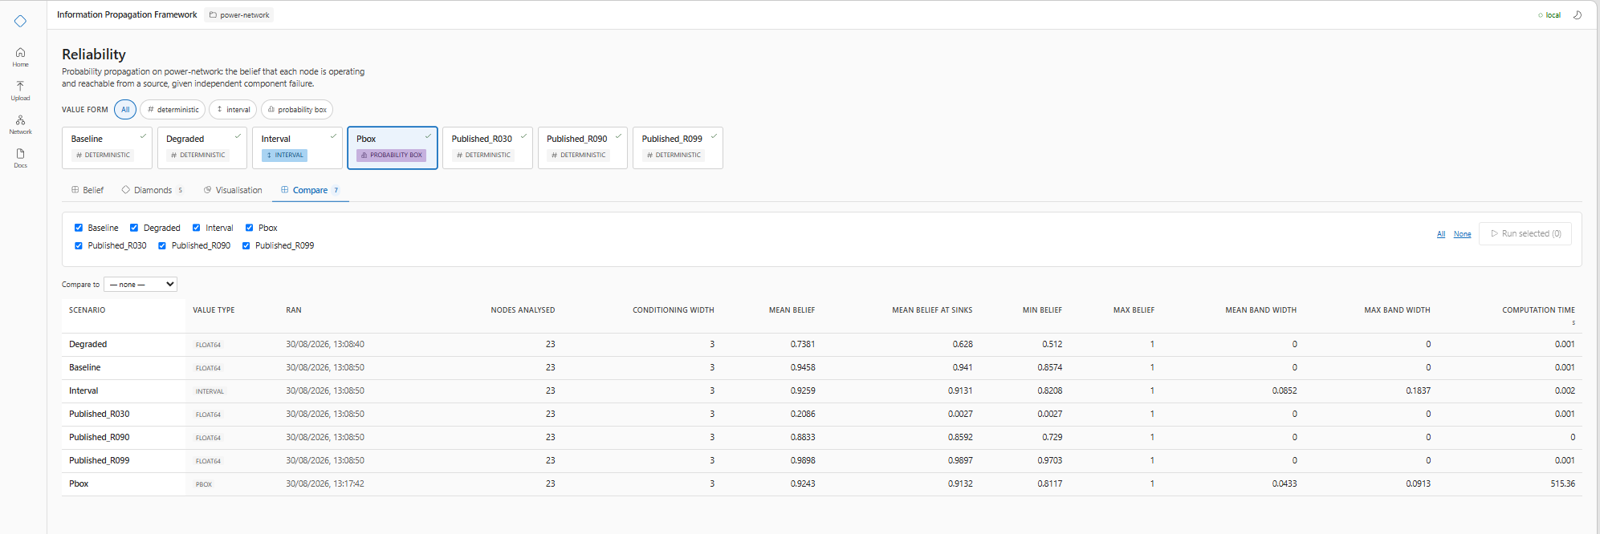
\includegraphics[width=\linewidth]{fig07_compare/fig07_compare.png}
  \caption{The Compare tab: scenario selection, the run control for scenarios not yet
  run, and the side-by-side table with a baseline selector.}
  \label{fig:fe-compare}
\end{figure}

\begin{figure}[htbp]
  \centering
  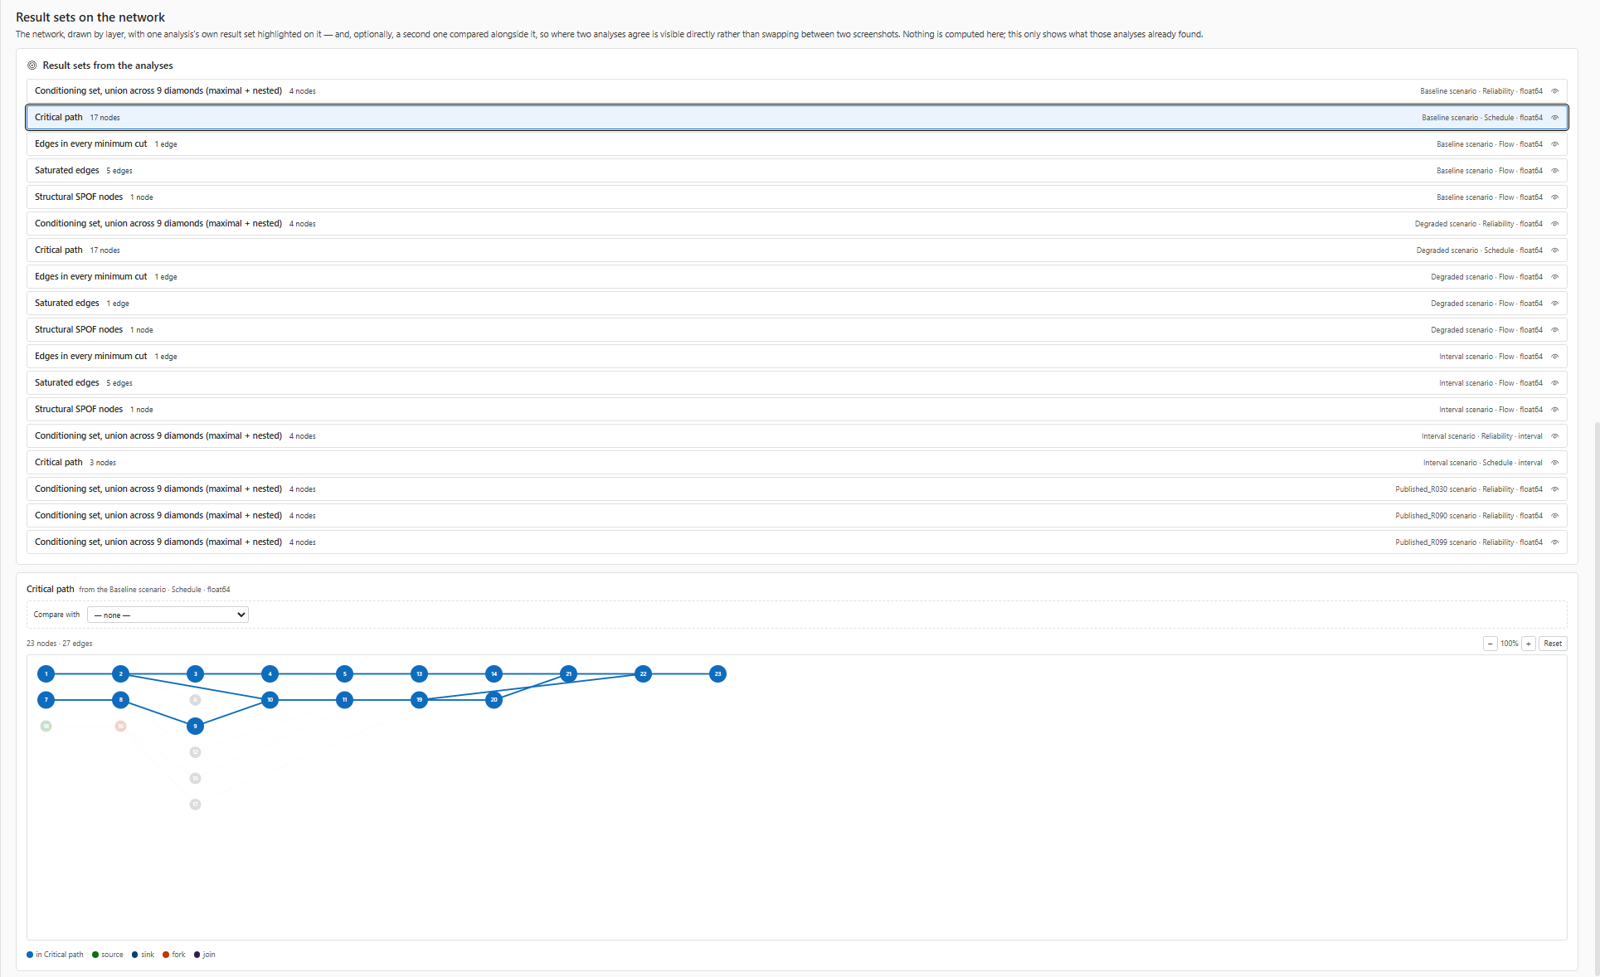
\includegraphics[width=\linewidth]{fig08_profile/fig08_profile.png}
  \caption{The system-profile page: the result sets available on the network, one
  selected and drawn by layer, with a second selectable for overlay.}
  \label{fig:fe-profile}
\end{figure}

\FloatBarrier
\section{What the Interface Enforces}
\label{sec:fe-rules}

The fourth requirement of Section~\ref{sec:fe-user}, that the screen shows what the package
computed and nothing else, is met by four rules that the interface applies everywhere, and
they are stated here with the reason for each.

A value keeps its form. A belief under an interval scenario is shown as a range wherever it
appears, and a belief under a probability-box scenario as its bounding summary, never as a
midpoint. One component, \texttt{ValueDisplay}, renders every value of every form in every
table and detail view, so that no view can invent its own rendering. The one exception is
stated on the screen: a few summary tiles, such as the mean belief, use a midpoint so that a
single summary number is possible, and each such tile says so in its label. A per-node value
is never flattened. The reason is Chapter~\ref{ch:probability-toolkit}: the range is the
result, and its midpoint is a number the toolkit never computed.

A result set is what the toolkit returned. The bottleneck table reports the edges in every
minimum cut as the flow toolkit computed them; the profile page draws a critical path as
the schedule toolkit reported it; no score, ranking or threshold is computed in the
interface. Where a table is sorted, the sort key is a field the toolkit returned. A number
computed in the interface would be a number the thesis has not validated.

Every result carries its method, since what a result guarantees depends on the method that
produced it (Chapter~\ref{ch:critical-path}). The schedule toolkit returns interval margins
from one of three methods, and the probability toolkit returns beliefs from an exact or a
decomposition-only call; in each case the response names the method, and the interface
shows the tag beside the result. A conservative enclosure and an exact range are never
displayed the same way, because a reader who cannot tell them apart cannot use either.

One analysis runs at a time. Because the propagation is single-threaded and its cache is
not locked (Chapter~\ref{ch:julia-package}), a second concurrent request would either wait
or, at worst, corrupt a shared store. The Compare tab therefore runs unrun scenarios in
sequence, and no view issues two requests to the server together.

However, one rule the interface does not yet enforce is recorded here because it was found
in use.
Probability-box propagation has a cost that grows steeply with the discretisation level of
the bounding functions, and Chapter~\ref{ch:probability-toolkit} recommends levels between
25 and 100 for networks of the scale the method suits. The server does not set the level,
so the library's own default of 200 applies to every request, which is the expensive end of
the range. A run on the 26-node KarlNetwork at that default ran for seventeen minutes and
blocked the single-threaded server, while the same run at level 50 completes in nine.
The interface exposes no control over the level, applies no default of its own, and gives
no estimate or warning before a run that may take minutes. What a user meets as
intractability is therefore a setting the theory chapter already documents, and the fix
is a control and a default in the interface, not a change to the method. It is listed in
Chapter~\ref{ch:conclusions}.

\section{Architecture}
\label{sec:fe-architecture}

The interface is an Angular application in an Nx workspace, built on Microsoft's Fluent
web components for its controls and on d3 for the network drawing. The workspace holds
eight projects: the application shell, which owns routing, the navigation rail and the
pages that are not toolkit-specific; five feature libraries, one per toolkit page
(reliability, which also carries the standalone Diamonds page, flow, schedule), one for
the system profile and one for the session-inputs editor; and three shared libraries, an
API client generated against the server's published contract, a data-access library
holding the scenario cache and the folder convention, and a presentational library of
cards, tables and the network graph.

Two dependency rules are enforced by the build, not by convention. A layer rule allows the
shell to depend on features, features on the shared libraries, and presentational
components only on other presentational components and the API client, never on data
access. Thus a component in the presentational library that needs a scenario's shape
declares a small structural type of its own. A scope rule allows a feature to depend on its
own scope and the shared scope only, so that no feature imports another feature; a view
that needs another toolkit's components, such as the standalone Diamonds page, lives inside
that toolkit's library. Both rules are checked by the linter on every build, which is how
the claim of Chapter~\ref{ch:main-intro} that the three analyses are independent is made
to hold in the interface as well as in the package.

The Fluent component set has no card, table or data-grid component, so the interface's
cards are its own and its tables are native HTML tables styled with the Fluent design
tokens. About forty components are registered once at start-up, and about fifty icons are
drawn from the Fluent system icon set.

Client and server share one machine. The server binds the loopback address and
accepts requests only from the interface's own origin, as Chapter~\ref{ch:julia-package}
describes, and the interface has no other network access. Every request names files by
their path in the session; no request carries the network in its body, and no file is
re-encoded on the way. Figure~\ref{fig:fe-deployment} shows the whole deployment inside the
boundary of the user's machine: the browser talks to the analysis service over HTTP on
localhost, and the service alone reaches the framework's modules and the session's files
and decomposition store. A local-first application in this sense keeps the usability of
the web without the custody question of Chapter~\ref{ch:lit-review}, since there is no
remote party to hold the data \cite{kleppmann2019local}.

\begin{figure}[htbp]
  \centering
  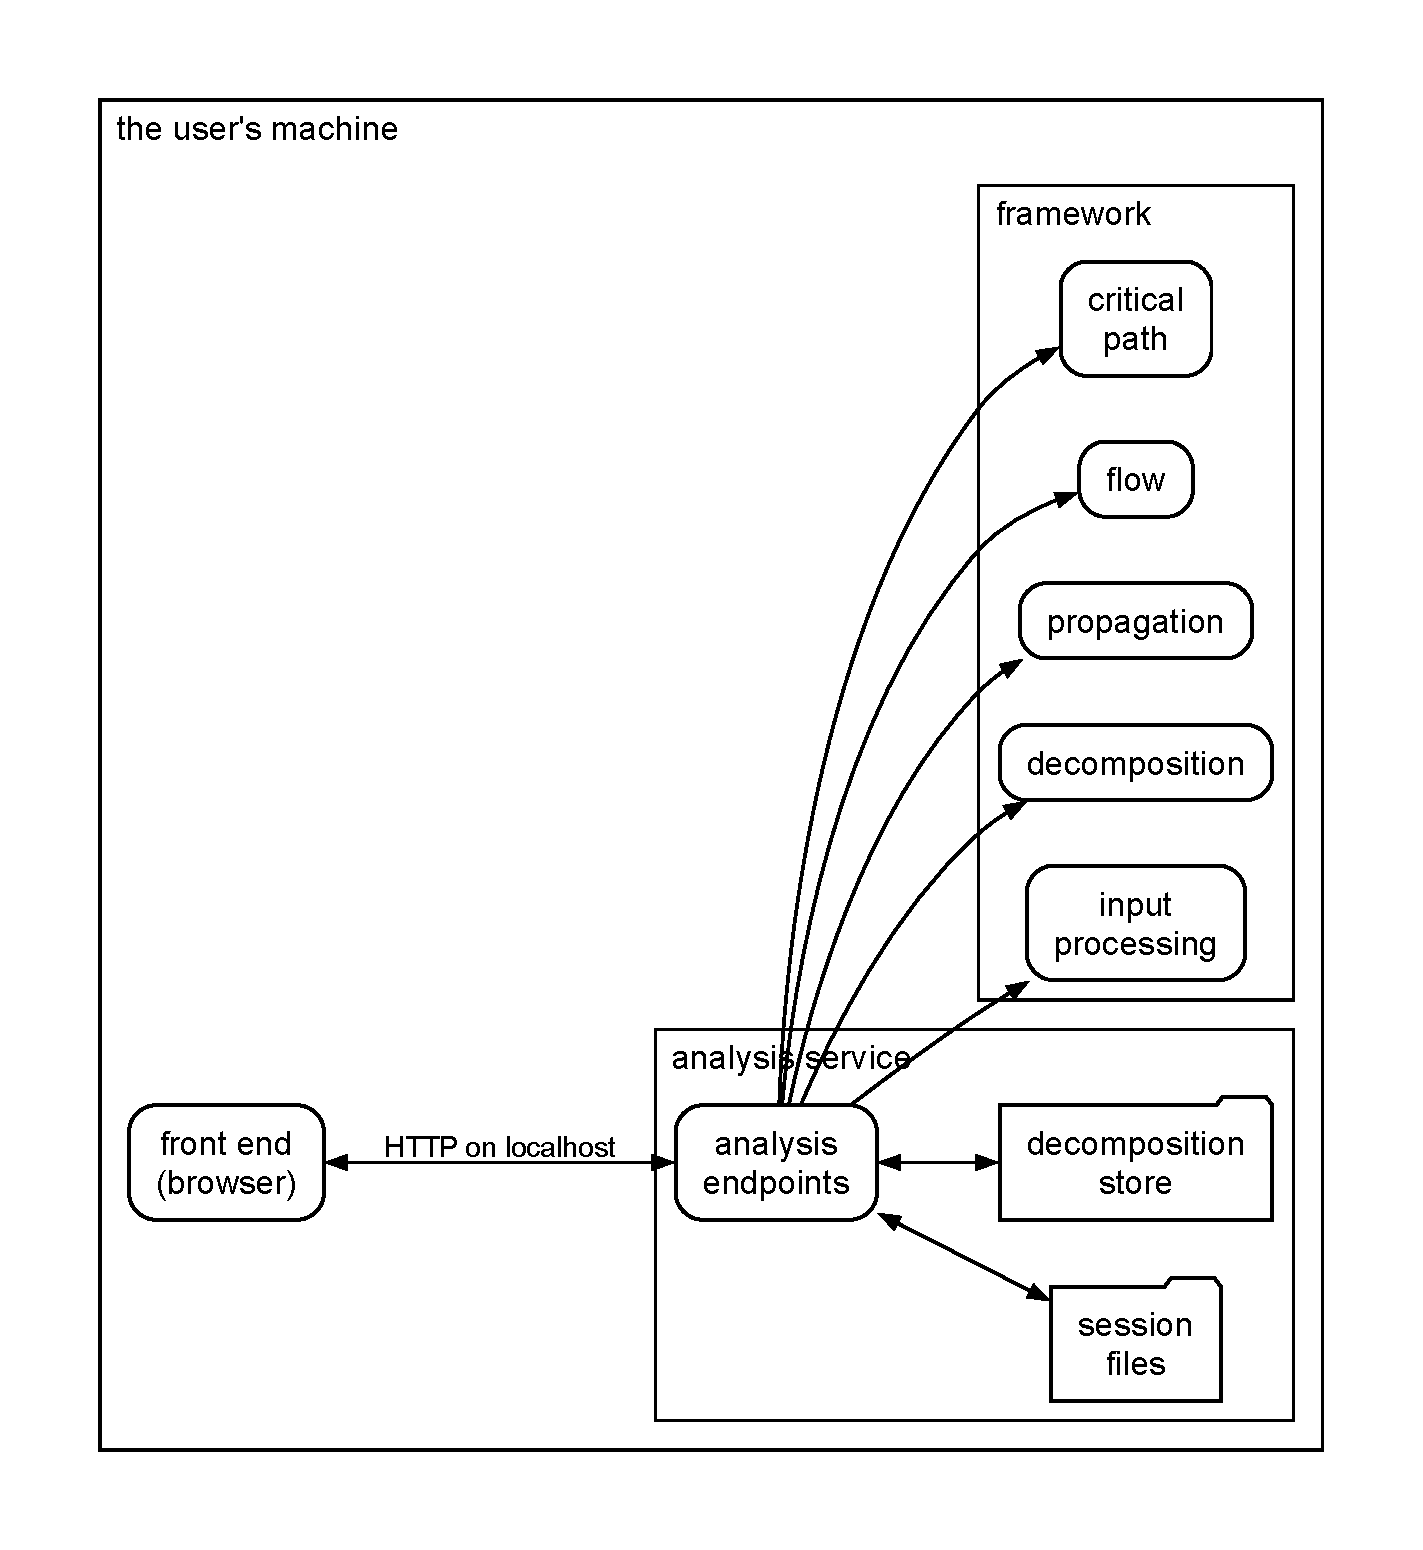
\includegraphics[width=0.85\linewidth]{fig09_architecture/fig09_architecture.pdf}
  \caption{The deployment, contained entirely within the user's machine. The front end
  reaches the analysis service over HTTP on localhost; the service alone calls the
  framework's modules and reads and writes the session's files and decomposition store.}
  \label{fig:fe-deployment}
\end{figure}

\section{The Contract as the Boundary}
\label{sec:fe-contract}

The boundary between interface and package is a written contract: an OpenAPI document,
version 2.0.0, describing fourteen endpoints, from which the interface's API client is
generated. Each analysis has one endpoint and one handler, and each endpoint takes a JSON
body naming the session and the files and returns a JSON response whose values keep their
form on the wire: a deterministic value is a number, an interval is an object with a lower
and an upper field, and a probability box is a fuller typed object. Because the same files
that the interface uploads are the files the package reads, anything the interface does can
be repeated from the command line against the same folder, and the case study of
Chapter~\ref{ch:integrated-case-study} records every server request and response beside its
screenshots for that reason.

The contract has changed once during the work, when three endpoints were renamed to match
the toolkit names of this thesis. The old names were kept as aliases, so the interface built
against the earlier contract continued to work while the client was regenerated. That is
the ordinary benefit of a published boundary, and it is recorded because it was tested.

\section{Evaluation}
\label{sec:fe-evaluation}

This interface has been used by its author and demonstrated to others, and it has not yet
been used independently by an engineer who does not program. Hence the evaluation that can
be offered is a task-based walkthrough, and it is labelled as such: it shows that the tasks
a user would set are reachable without code, and it does not show how a user found them.

The tasks are the ones a planner with a system model would set. Load a model that exists as
an edge list and three input files. See whether the structure was read as intended. Find
the belief at each demand point under the current component data, and under a stated range
on that data. Find which reconvergence in the network carries the uncertainty, and study it
alone. Find the deliverable throughput and the binding cut, and what fails first. Find the
completion time of a dependent sequence and which activities are certainly critical under
duration uncertainty. Compare two operating cases. See where the schedule's critical path
and the flow's binding cut coincide.

Every one of these is a click sequence in Section~\ref{sec:fe-workflow}, and every result
it produces is a result of Chapters~\ref{ch:probability-toolkit}
to~\ref{ch:critical-path} in the form those chapters state. The demonstration of the
sequence on a real network, with every request and response recorded, is
Chapter~\ref{ch:integrated-case-study}. However, the walkthrough cannot show the time a new
user takes, where the labels are unclear, or which of the four rules of
Section~\ref{sec:fe-rules} a user notices; that is the study that remains to be done, and
it is listed in Chapter~\ref{ch:conclusions}.

\section{Limitations}
\label{sec:fe-limitations}

The interface has no control over the probability-box discretisation level and no warning
before a long run, as Section~\ref{sec:fe-rules} records. It has no user study behind it.
It accepts the two structure formats of Chapter~\ref{ch:system-model} and no domain format,
so a user with an EPANET or MATPOWER file converts it first. It runs one analysis at a
time. The session is a folder on disk and there is no export beyond the response JSON,
which the user can save from the browser. Finally, the interface is a client of the
package, so every limit of the package, single-threaded propagation, no probability-box
schedule, no interval flow, is a limit of the interface as well.

\section{Summary}
\label{sec:fe-summary}

An engineer who does not program can run the three toolkits on a system model by uploading
the files the package reads and pressing a button, on a machine the model never leaves. The
interface shows what the package computed and enforces that in four rules: a value keeps
its form, a result set is what the toolkit returned, every result carries its method, and
one analysis runs at a time. It is built as an Angular workspace whose module boundaries
are checked by the build, against a published contract from which its client is generated,
so that anything done in the interface can be repeated at the command line. One cost
control is missing and has been located. The interface has been demonstrated and not yet
studied in use, and its application to a real network follows in the next chapter.

\ifdefined\maindoc
\else
\printbibliography
\end{document}
\fi